% Options for packages loaded elsewhere
\PassOptionsToPackage{unicode}{hyperref}
\PassOptionsToPackage{hyphens}{url}
%
\documentclass[
]{article}
\usepackage{amsmath,amssymb}
\usepackage{iftex}
\ifPDFTeX
  \usepackage[T1]{fontenc}
  \usepackage[utf8]{inputenc}
  \usepackage{textcomp} % provide euro and other symbols
\else % if luatex or xetex
  \usepackage{unicode-math} % this also loads fontspec
  \defaultfontfeatures{Scale=MatchLowercase}
  \defaultfontfeatures[\rmfamily]{Ligatures=TeX,Scale=1}
\fi
\usepackage{lmodern}
\ifPDFTeX\else
  % xetex/luatex font selection
\fi
% Use upquote if available, for straight quotes in verbatim environments
\IfFileExists{upquote.sty}{\usepackage{upquote}}{}
\IfFileExists{microtype.sty}{% use microtype if available
  \usepackage[]{microtype}
  \UseMicrotypeSet[protrusion]{basicmath} % disable protrusion for tt fonts
}{}
\makeatletter
\@ifundefined{KOMAClassName}{% if non-KOMA class
  \IfFileExists{parskip.sty}{%
    \usepackage{parskip}
  }{% else
    \setlength{\parindent}{0pt}
    \setlength{\parskip}{6pt plus 2pt minus 1pt}}
}{% if KOMA class
  \KOMAoptions{parskip=half}}
\makeatother
\usepackage{xcolor}
\usepackage[margin=1in]{geometry}
\usepackage{color}
\usepackage{fancyvrb}
\newcommand{\VerbBar}{|}
\newcommand{\VERB}{\Verb[commandchars=\\\{\}]}
\DefineVerbatimEnvironment{Highlighting}{Verbatim}{commandchars=\\\{\}}
% Add ',fontsize=\small' for more characters per line
\usepackage{framed}
\definecolor{shadecolor}{RGB}{248,248,248}
\newenvironment{Shaded}{\begin{snugshade}}{\end{snugshade}}
\newcommand{\AlertTok}[1]{\textcolor[rgb]{0.94,0.16,0.16}{#1}}
\newcommand{\AnnotationTok}[1]{\textcolor[rgb]{0.56,0.35,0.01}{\textbf{\textit{#1}}}}
\newcommand{\AttributeTok}[1]{\textcolor[rgb]{0.13,0.29,0.53}{#1}}
\newcommand{\BaseNTok}[1]{\textcolor[rgb]{0.00,0.00,0.81}{#1}}
\newcommand{\BuiltInTok}[1]{#1}
\newcommand{\CharTok}[1]{\textcolor[rgb]{0.31,0.60,0.02}{#1}}
\newcommand{\CommentTok}[1]{\textcolor[rgb]{0.56,0.35,0.01}{\textit{#1}}}
\newcommand{\CommentVarTok}[1]{\textcolor[rgb]{0.56,0.35,0.01}{\textbf{\textit{#1}}}}
\newcommand{\ConstantTok}[1]{\textcolor[rgb]{0.56,0.35,0.01}{#1}}
\newcommand{\ControlFlowTok}[1]{\textcolor[rgb]{0.13,0.29,0.53}{\textbf{#1}}}
\newcommand{\DataTypeTok}[1]{\textcolor[rgb]{0.13,0.29,0.53}{#1}}
\newcommand{\DecValTok}[1]{\textcolor[rgb]{0.00,0.00,0.81}{#1}}
\newcommand{\DocumentationTok}[1]{\textcolor[rgb]{0.56,0.35,0.01}{\textbf{\textit{#1}}}}
\newcommand{\ErrorTok}[1]{\textcolor[rgb]{0.64,0.00,0.00}{\textbf{#1}}}
\newcommand{\ExtensionTok}[1]{#1}
\newcommand{\FloatTok}[1]{\textcolor[rgb]{0.00,0.00,0.81}{#1}}
\newcommand{\FunctionTok}[1]{\textcolor[rgb]{0.13,0.29,0.53}{\textbf{#1}}}
\newcommand{\ImportTok}[1]{#1}
\newcommand{\InformationTok}[1]{\textcolor[rgb]{0.56,0.35,0.01}{\textbf{\textit{#1}}}}
\newcommand{\KeywordTok}[1]{\textcolor[rgb]{0.13,0.29,0.53}{\textbf{#1}}}
\newcommand{\NormalTok}[1]{#1}
\newcommand{\OperatorTok}[1]{\textcolor[rgb]{0.81,0.36,0.00}{\textbf{#1}}}
\newcommand{\OtherTok}[1]{\textcolor[rgb]{0.56,0.35,0.01}{#1}}
\newcommand{\PreprocessorTok}[1]{\textcolor[rgb]{0.56,0.35,0.01}{\textit{#1}}}
\newcommand{\RegionMarkerTok}[1]{#1}
\newcommand{\SpecialCharTok}[1]{\textcolor[rgb]{0.81,0.36,0.00}{\textbf{#1}}}
\newcommand{\SpecialStringTok}[1]{\textcolor[rgb]{0.31,0.60,0.02}{#1}}
\newcommand{\StringTok}[1]{\textcolor[rgb]{0.31,0.60,0.02}{#1}}
\newcommand{\VariableTok}[1]{\textcolor[rgb]{0.00,0.00,0.00}{#1}}
\newcommand{\VerbatimStringTok}[1]{\textcolor[rgb]{0.31,0.60,0.02}{#1}}
\newcommand{\WarningTok}[1]{\textcolor[rgb]{0.56,0.35,0.01}{\textbf{\textit{#1}}}}
\usepackage{longtable,booktabs,array}
\usepackage{calc} % for calculating minipage widths
% Correct order of tables after \paragraph or \subparagraph
\usepackage{etoolbox}
\makeatletter
\patchcmd\longtable{\par}{\if@noskipsec\mbox{}\fi\par}{}{}
\makeatother
% Allow footnotes in longtable head/foot
\IfFileExists{footnotehyper.sty}{\usepackage{footnotehyper}}{\usepackage{footnote}}
\makesavenoteenv{longtable}
\usepackage{graphicx}
\makeatletter
\def\maxwidth{\ifdim\Gin@nat@width>\linewidth\linewidth\else\Gin@nat@width\fi}
\def\maxheight{\ifdim\Gin@nat@height>\textheight\textheight\else\Gin@nat@height\fi}
\makeatother
% Scale images if necessary, so that they will not overflow the page
% margins by default, and it is still possible to overwrite the defaults
% using explicit options in \includegraphics[width, height, ...]{}
\setkeys{Gin}{width=\maxwidth,height=\maxheight,keepaspectratio}
% Set default figure placement to htbp
\makeatletter
\def\fps@figure{htbp}
\makeatother
\setlength{\emergencystretch}{3em} % prevent overfull lines
\providecommand{\tightlist}{%
  \setlength{\itemsep}{0pt}\setlength{\parskip}{0pt}}
\setcounter{secnumdepth}{-\maxdimen} % remove section numbering
<!--radix_placeholder_navigation_in_header-->
<meta name="distill:offset" content=""/>

<script type="application/javascript">

  window.headroom_prevent_pin = false;

  window.document.addEventListener("DOMContentLoaded", function (event) {

    // initialize headroom for banner
    var header = $('header').get(0);
    var headerHeight = header.offsetHeight;
    var headroom = new Headroom(header, {
      tolerance: 5,
      onPin : function() {
        if (window.headroom_prevent_pin) {
          window.headroom_prevent_pin = false;
          headroom.unpin();
        }
      }
    });
    headroom.init();
    if(window.location.hash)
      headroom.unpin();
    $(header).addClass('headroom--transition');

    // offset scroll location for banner on hash change
    // (see: https://github.com/WickyNilliams/headroom.js/issues/38)
    window.addEventListener("hashchange", function(event) {
      window.scrollTo(0, window.pageYOffset - (headerHeight + 25));
    });

    // responsive menu
    $('.distill-site-header').each(function(i, val) {
      var topnav = $(this);
      var toggle = topnav.find('.nav-toggle');
      toggle.on('click', function() {
        topnav.toggleClass('responsive');
      });
    });

    // nav dropdowns
    $('.nav-dropbtn').click(function(e) {
      $(this).next('.nav-dropdown-content').toggleClass('nav-dropdown-active');
      $(this).parent().siblings('.nav-dropdown')
         .children('.nav-dropdown-content').removeClass('nav-dropdown-active');
    });
    $("body").click(function(e){
      $('.nav-dropdown-content').removeClass('nav-dropdown-active');
    });
    $(".nav-dropdown").click(function(e){
      e.stopPropagation();
    });
  });
</script>

<style type="text/css">

/* Theme (user-documented overrideables for nav appearance) */

.distill-site-nav {
  color: rgba(255, 255, 255, 0.8);
  background-color: #0F2E3D;
  font-size: 15px;
  font-weight: 300;
}

.distill-site-nav a {
  color: inherit;
  text-decoration: none;
}

.distill-site-nav a:hover {
  color: white;
}

@media print {
  .distill-site-nav {
    display: none;
  }
}

.distill-site-header {

}

.distill-site-footer {

}


/* Site Header */

.distill-site-header {
  width: 100%;
  box-sizing: border-box;
  z-index: 3;
}

.distill-site-header .nav-left {
  display: inline-block;
  margin-left: 8px;
}

@media screen and (max-width: 768px) {
  .distill-site-header .nav-left {
    margin-left: 0;
  }
}


.distill-site-header .nav-right {
  float: right;
  margin-right: 8px;
}

.distill-site-header a,
.distill-site-header .title {
  display: inline-block;
  text-align: center;
  padding: 14px 10px 14px 10px;
}

.distill-site-header .title {
  font-size: 18px;
  min-width: 150px;
}

.distill-site-header .logo {
  padding: 0;
}

.distill-site-header .logo img {
  display: none;
  max-height: 20px;
  width: auto;
  margin-bottom: -4px;
}

.distill-site-header .nav-image img {
  max-height: 18px;
  width: auto;
  display: inline-block;
  margin-bottom: -3px;
}



@media screen and (min-width: 1000px) {
  .distill-site-header .logo img {
    display: inline-block;
  }
  .distill-site-header .nav-left {
    margin-left: 20px;
  }
  .distill-site-header .nav-right {
    margin-right: 20px;
  }
  .distill-site-header .title {
    padding-left: 12px;
  }
}


.distill-site-header .nav-toggle {
  display: none;
}

.nav-dropdown {
  display: inline-block;
  position: relative;
}

.nav-dropdown .nav-dropbtn {
  border: none;
  outline: none;
  color: rgba(255, 255, 255, 0.8);
  padding: 16px 10px;
  background-color: transparent;
  font-family: inherit;
  font-size: inherit;
  font-weight: inherit;
  margin: 0;
  margin-top: 1px;
  z-index: 2;
}

.nav-dropdown-content {
  display: none;
  position: absolute;
  background-color: white;
  min-width: 200px;
  border: 1px solid rgba(0,0,0,0.15);
  border-radius: 4px;
  box-shadow: 0px 8px 16px 0px rgba(0,0,0,0.1);
  z-index: 1;
  margin-top: 2px;
  white-space: nowrap;
  padding-top: 4px;
  padding-bottom: 4px;
}

.nav-dropdown-content hr {
  margin-top: 4px;
  margin-bottom: 4px;
  border: none;
  border-bottom: 1px solid rgba(0, 0, 0, 0.1);
}

.nav-dropdown-active {
  display: block;
}

.nav-dropdown-content a, .nav-dropdown-content .nav-dropdown-header {
  color: black;
  padding: 6px 24px;
  text-decoration: none;
  display: block;
  text-align: left;
}

.nav-dropdown-content .nav-dropdown-header {
  display: block;
  padding: 5px 24px;
  padding-bottom: 0;
  text-transform: uppercase;
  font-size: 14px;
  color: #999999;
  white-space: nowrap;
}

.nav-dropdown:hover .nav-dropbtn {
  color: white;
}

.nav-dropdown-content a:hover {
  background-color: #ddd;
  color: black;
}

.nav-right .nav-dropdown-content {
  margin-left: -45%;
  right: 0;
}

@media screen and (max-width: 768px) {
  .distill-site-header a, .distill-site-header .nav-dropdown  {display: none;}
  .distill-site-header a.nav-toggle {
    float: right;
    display: block;
  }
  .distill-site-header .title {
    margin-left: 0;
  }
  .distill-site-header .nav-right {
    margin-right: 0;
  }
  .distill-site-header {
    overflow: hidden;
  }
  .nav-right .nav-dropdown-content {
    margin-left: 0;
  }
}


@media screen and (max-width: 768px) {
  .distill-site-header.responsive {position: relative; min-height: 500px; }
  .distill-site-header.responsive a.nav-toggle {
    position: absolute;
    right: 0;
    top: 0;
  }
  .distill-site-header.responsive a,
  .distill-site-header.responsive .nav-dropdown {
    display: block;
    text-align: left;
  }
  .distill-site-header.responsive .nav-left,
  .distill-site-header.responsive .nav-right {
    width: 100%;
  }
  .distill-site-header.responsive .nav-dropdown {float: none;}
  .distill-site-header.responsive .nav-dropdown-content {position: relative;}
  .distill-site-header.responsive .nav-dropdown .nav-dropbtn {
    display: block;
    width: 100%;
    text-align: left;
  }
}

/* Site Footer */

.distill-site-footer {
  width: 100%;
  overflow: hidden;
  box-sizing: border-box;
  z-index: 3;
  margin-top: 30px;
  padding-top: 30px;
  padding-bottom: 30px;
  text-align: center;
}

/* Headroom */

d-title {
  padding-top: 6rem;
}

@media print {
  d-title {
    padding-top: 4rem;
  }
}

.headroom {
  z-index: 1000;
  position: fixed;
  top: 0;
  left: 0;
  right: 0;
}

.headroom--transition {
  transition: all .4s ease-in-out;
}

.headroom--unpinned {
  top: -100px;
}

.headroom--pinned {
  top: 0;
}

/* adjust viewport for navbar height */
/* helps vertically center bootstrap (non-distill) content */
.min-vh-100 {
  min-height: calc(100vh - 100px) !important;
}

</style>

<script src="site_libs/jquery-3.6.0/jquery-3.6.0.min.js"></script>
<link href="site_libs/font-awesome-5.1.0/css/all.css" rel="stylesheet"/>
<link href="site_libs/font-awesome-5.1.0/css/v4-shims.css" rel="stylesheet"/>
<script src="site_libs/headroom-0.9.4/headroom.min.js"></script>
<!--/radix_placeholder_navigation_in_header-->
<!--radix_placeholder_site_in_header-->
<!--/radix_placeholder_site_in_header-->

<style type="text/css">
body {
  padding-top: 60px;
}
</style>
<style type="text/css">
/* base variables */

/* Edit the CSS properties in this file to create a custom
   Distill theme. Only edit values in the right column
   for each row; values shown are the CSS defaults.
   To return any property to the default,
   you may set its value to: unset
   All rows must end with a semi-colon.                      */

/* Optional: embed custom fonts here with `@import`          */
/* This must remain at the top of this file.                 */



html {
  /*-- Main font sizes --*/
  --title-size:      50px;
  --body-size:       1.06rem;
  --code-size:       14px;
  --aside-size:      12px;
  --fig-cap-size:    13px;
  /*-- Main font colors --*/
  --title-color:     #000000;
  --header-color:    rgba(0, 0, 0, 0.8);
  --body-color:      rgba(0, 0, 0, 0.8);
  --aside-color:     rgba(0, 0, 0, 0.6);
  --fig-cap-color:   rgba(0, 0, 0, 0.6);
  /*-- Specify custom fonts ~~~ must be imported above   --*/
  --heading-font:    sans-serif;
  --mono-font:       monospace;
  --body-font:       sans-serif;
  --navbar-font:     sans-serif;  /* websites + blogs only */
}

/*-- ARTICLE METADATA --*/
d-byline {
  --heading-size:    0.6rem;
  --heading-color:   rgba(0, 0, 0, 0.5);
  --body-size:       0.8rem;
  --body-color:      rgba(0, 0, 0, 0.8);
}

/*-- ARTICLE TABLE OF CONTENTS --*/
.d-contents {
  --heading-size:    18px;
  --contents-size:   13px;
}

/*-- ARTICLE APPENDIX --*/
d-appendix {
  --heading-size:    15px;
  --heading-color:   rgba(0, 0, 0, 0.65);
  --text-size:       0.8em;
  --text-color:      rgba(0, 0, 0, 0.5);
}

/*-- WEBSITE HEADER + FOOTER --*/
/* These properties only apply to Distill sites and blogs  */

.distill-site-header {
  --title-size:       18px;
  --text-color:       rgba(255, 255, 255, 0.8);
  --text-size:        15px;
  --hover-color:      white;
  --bkgd-color:       #0F2E3D;
}

.distill-site-footer {
  --text-color:       rgba(255, 255, 255, 0.8);
  --text-size:        15px;
  --hover-color:      white;
  --bkgd-color:       #0F2E3D;
}

/*-- Additional custom styles --*/
/* Add any additional CSS rules below                      */
</style>
<style type="text/css">
/* base variables */

/* Edit the CSS properties in this file to create a custom
   Distill theme. Only edit values in the right column
   for each row; values shown are the CSS defaults.
   To return any property to the default,
   you may set its value to: unset
   All rows must end with a semi-colon.                      */

/* Optional: embed custom fonts here with `@import`          */
/* This must remain at the top of this file.                 */
@import url('https://fonts.googleapis.com/css2?family=Lato');
@import url('https://fonts.googleapis.com/css2?family=Lora');


html {
  /*-- Main font sizes --*/
  --title-size:      50px;
  --body-size:       1.06rem;
  --code-size:       13px;
  --aside-size:      12px;
  --fig-cap-size:    12px;
  /*-- Main font colors --*/
  --title-color:     rgba(29, 71, 73, 0.9);
  --header-color:    rgba(29, 71, 73, 0.9);
  --body-color:      rgba(0, 0, 0, 0.8);
  --aside-color:     rgba(0, 0, 0, 0.6);
  --fig-cap-color:   rgba(0, 0, 0, 0.6);
  --hover-color:     rgba(29, 71, 73, 0.5);
  /*-- Specify custom fonts ~~~ must be imported above   --*/
  --heading-font:    "Lato", sans-serif;
  --body-font:       "Lora", serif;
  --navbar-font:     "Lato", sans-serif;  /* websites + blogs only */
}

/*-- ARTICLE METADATA --*/
d-byline {
  --heading-size:    0.6rem;
  --heading-color:   rgba(0, 0, 0, 0.5);
  --body-size:       0.8rem;
  --body-color:      rgba(0, 0, 0, 0.8);
}

/*-- ARTICLE TABLE OF CONTENTS --*/
.d-contents {
  --heading-size:    18px;
  --contents-size:   13px;
}

/*-- ARTICLE APPENDIX --*/
d-appendix {
  --heading-size:    15px;
  --heading-color:   rgba(0, 0, 0, 0.65);
  --text-size:       0.8em;
  --text-color:      rgba(0, 0, 0, 0.5);
}

/*-- WEBSITE HEADER + FOOTER --*/
/* These properties only apply to Distill sites and blogs  */

.distill-site-header {
  --font-family:      'Lato', sans-serif;
  --title-size:       21px;
  --text-color:       rgba(29, 71, 73, 0.9);
  --text-size:        18px;
  --hover-color:      rgba(29, 71, 73, 0.5);
  --bkgd-color:       rgba(255, 255, 255, 0.8);
  font-variant:       small-caps;
}

.nav-dropdown .nav-dropbtn {
  font-variant: small-caps;
}

.distill-site-footer {
  --text-color:       rgba(10, 10, 10, 0.8);
  --text-size:        15px;
  --hover-color:      white;
  --bkgd-color:       rgba(240, 240, 240, 0.8); 
}

/*-- Additional custom styles --*/
/* Add any additional CSS rules below                      */

/* Postcard headers */
h1, h2, h3 {
  color:              rgba(29, 71, 73, 0.9);
  font-variant:       small-caps;
}

p {
  color:              rgba(0, 0, 0, 0.8);
}

a {
	color:              rgba(29, 71, 73, 0.9);
}

a:hover {
	color:              rgba(29, 71, 73, 0.5);
}

/* Buttons on postcard */
.btn-outline-dark {
  color:              rgba(29, 71, 73, 0.9);
  border-color:       rgba(29, 71, 73, 0.9);
}

.btn-outline-dark:hover {
  background-color:   rgba(29, 71, 73, 0.9);
  color:              white;
}

/*body {
  background-color: rgba(249, 250, 247, 0.8);
}*/</style>
<style type="text/css">
/* base style */

/* FONT FAMILIES */

:root {
  --heading-default: -apple-system, BlinkMacSystemFont, "Segoe UI", Roboto, Oxygen, Ubuntu, Cantarell, "Fira Sans", "Droid Sans", "Helvetica Neue", Arial, sans-serif;
  --mono-default: Consolas, Monaco, 'Andale Mono', 'Ubuntu Mono', monospace;
  --body-default: -apple-system, BlinkMacSystemFont, "Segoe UI", Roboto, Oxygen, Ubuntu, Cantarell, "Fira Sans", "Droid Sans", "Helvetica Neue", Arial, sans-serif;
}

body,
.posts-list .post-preview p,
.posts-list .description p {
  font-family: var(--body-font), var(--body-default);
}

h1, h2, h3, h4, h5, h6,
.posts-list .post-preview h2,
.posts-list .description h2 {
  font-family: var(--heading-font), var(--heading-default);
}

d-article div.sourceCode code,
d-article pre code {
  font-family: var(--mono-font), var(--mono-default);
}


/*-- TITLE --*/
d-title h1,
.posts-list > h1 {
  color: var(--title-color, black);
}

d-title h1 {
  font-size: var(--title-size, 50px);
}

/*-- HEADERS --*/
d-article h1,
d-article h2,
d-article h3,
d-article h4,
d-article h5,
d-article h6 {
  color: var(--header-color, rgba(0, 0, 0, 0.8));
}

/*-- BODY --*/
d-article > p,  /* only text inside of <p> tags */
d-article > ul, /* lists */
d-article > ol {
  color: var(--body-color, rgba(0, 0, 0, 0.8));
  font-size: var(--body-size, 1.06rem);
}


/*-- CODE --*/
d-article div.sourceCode code,
d-article pre code {
  font-size: var(--code-size, 14px);
}

/*-- ASIDE --*/
d-article aside {
  font-size: var(--aside-size, 12px);
  color: var(--aside-color, rgba(0, 0, 0, 0.6));
}

/*-- FIGURE CAPTIONS --*/
figure .caption,
figure figcaption,
.figure .caption {
  font-size: var(--fig-cap-size, 13px);
  color: var(--fig-cap-color, rgba(0, 0, 0, 0.6));
}

/*-- METADATA --*/
d-byline h3 {
  font-size: var(--heading-size, 0.6rem);
  color: var(--heading-color, rgba(0, 0, 0, 0.5));
}

d-byline {
  font-size: var(--body-size, 0.8rem);
  color: var(--body-color, rgba(0, 0, 0, 0.8));
}

d-byline a,
d-article d-byline a {
  color: var(--body-color, rgba(0, 0, 0, 0.8));
}

/*-- TABLE OF CONTENTS --*/
.d-contents nav h3 {
  font-size: var(--heading-size, 18px);
}

.d-contents nav a {
  font-size: var(--contents-size, 13px);
}

/*-- APPENDIX --*/
d-appendix h3 {
  font-size: var(--heading-size, 15px);
  color: var(--heading-color, rgba(0, 0, 0, 0.65));
}

d-appendix {
  font-size: var(--text-size, 0.8em);
  color: var(--text-color, rgba(0, 0, 0, 0.5));
}

d-appendix d-footnote-list a.footnote-backlink {
  color: var(--text-color, rgba(0, 0, 0, 0.5));
}

/*-- WEBSITE HEADER + FOOTER --*/
.distill-site-header .title {
  font-size: var(--title-size, 18px);
  font-family: var(--navbar-font), var(--heading-default);
}

.distill-site-header a,
.nav-dropdown .nav-dropbtn {
  font-family: var(--navbar-font), var(--heading-default);
}

.nav-dropdown .nav-dropbtn {
  color: var(--text-color, rgba(255, 255, 255, 0.8));
  font-size: var(--text-size, 15px);
}

.distill-site-header a:hover,
.nav-dropdown:hover .nav-dropbtn {
  color: var(--hover-color, white);
}

.distill-site-header {
  font-size: var(--text-size, 15px);
  color: var(--text-color, rgba(255, 255, 255, 0.8));
  background-color: var(--bkgd-color, #0F2E3D);
}

.distill-site-footer {
  font-size: var(--text-size, 15px);
  color: var(--text-color, rgba(255, 255, 255, 0.8));
  background-color: var(--bkgd-color, #0F2E3D);
}

.distill-site-footer a:hover {
  color: var(--hover-color, white);
}</style>
\ifLuaTeX
  \usepackage{selnolig}  % disable illegal ligatures
\fi
\IfFileExists{bookmark.sty}{\usepackage{bookmark}}{\usepackage{hyperref}}
\IfFileExists{xurl.sty}{\usepackage{xurl}}{} % add URL line breaks if available
\urlstyle{same}
\hypersetup{
  pdftitle={Simulations exogenous shocks},
  hidelinks,
  pdfcreator={LaTeX via pandoc}}

\title{Simulations exogenous shocks}
\author{}
\date{\vspace{-2.5em}}

\begin{document}
\maketitle

<!--radix_placeholder_navigation_before_body-->
<header class="header header--fixed" role="banner">
<nav class="distill-site-nav distill-site-header">
<div class="nav-left">
<a href="index.html" class="title">Causal Exaggeration</a>
</div>
<div class="nav-right">
<a href="causal_exaggeration_paper.pdf">Paper</a>
<a href="summary.html">Summary</a>
<a href="intuition.html">Intuition</a>
<a href="maths.html">Maths</a>
<div class="nav-dropdown">
<button class="nav-dropbtn">
Simulations
 
<span class="down-arrow">&#x25BE;</span>
</button>
<div class="nav-dropdown-content">
<a href="RDD.html">RDD</a>
<a href="IV.html">IV</a>
<a href="Matching.html">Matching</a>
<a href="DID.html">DiD / Event study</a>
<a href="crosscutting-issues.html">Crosscutting issues</a>
</div>
</div>
<a href="reporting.html">Reporting</a>
<a href="https://github.com/vincentbagilet/causal_exaggeration" aria-label="Link to source">
<i class="fab fa-github" aria-hidden="true"></i>
</a>
<a href="javascript:void(0);" class="nav-toggle">&#9776;</a>
</div>
</nav>
</header>
<!--/radix_placeholder_navigation_before_body-->

<!--radix_placeholder_site_before_body-->
<!--/radix_placeholder_site_before_body-->

\hypertarget{summary-and-intuition}{%
\subsection{Summary and intuition}\label{summary-and-intuition}}

\hypertarget{a-trade-off-mediaed-by-the-number-of-treated-observations}{%
\subsubsection{A trade-off mediaed by the number of treated
observations}\label{a-trade-off-mediaed-by-the-number-of-treated-observations}}

In the case of studies using exogenous shocks, a confounding /
exaggeration trade-off is mediated by the number of treated
observations. In some settings, while the number of observations is
large, the number of events might be limited. Pinpointing exogenous
shocks is never easy and we are sometimes only able to find a limited
number of occurrences of this shock or shocks affecting a small portion
of the population. More precisely, the number of observations with a non
null treatment status might be small. In this instance, the variation
available to identify the treatment is limited, possibly leading power
to be low and exaggeration issues to arise.

\hypertarget{intuition-to-explain-the-variation-of-power-with-the-number-of-treated-observations}{%
\subsubsection{Intuition to explain the variation of power with the
number of treated
observations}\label{intuition-to-explain-the-variation-of-power-with-the-number-of-treated-observations}}

The number of treated observations can be decomposed into two parts: the
total number of observations times the proportion of observations in the
treated group. Of course, if one reduces the total sample size,
precision and thus statistical power will decrease. At a fixed total
sample size and as commonly discussed in the Randomized Control Trial
literature, statistical power is maximized when the proportion of
treated observations is equal to the proportion of untreated ones. If we
consider a fixed number of observations, decreasing the proportion of
treated observations below 0.5 will decrease precision and power. The
intuition for this relationship can be given by studying the simple
formula for the standard error of the difference between the mean of the
outcome for the control and treatment groups. It does not represent the
actual standard error of the DiD estimator but can be useful to get an
intuition for this trade-off. The formula is the following:

\[se_{\bar{y_T} - \bar{y_c}} = \sqrt{\dfrac{\sigma_T^2}{n_T} + \dfrac{\sigma_C^2}{n_C}}\]
where \(n_T\) and \(n_C\) are the number of observation in the treated
group and the control group respectively and \(\sigma_T\) and
\(\sigma_C\) the standard deviations of the outcome in the treated group
and the control group respectively. In many cases, we can assume that
\(\sigma_T = \sigma_C = \sigma\). Under this assumption we have:

\[se_{\bar{y_T} - \bar{y_c}} = \dfrac{\sigma}{\sqrt{n}} \times \sqrt{\dfrac{1}{p_T(1-p_T)}}\]
where \(n\) is the total number of observations (\(n = n_T + n_C\)) and
\(p_T\) the proportion of treated observations.

From this simple formula it is obvious that the standard error of
interest increases when \(n\) decreases and that, for \(n\) constant, it
is minimized when the proportion of treated is 0.5. Since statistical
power is a decreasing function of the variance of an estimator, it will
decrease when the proportion of treated diverges from 0.5.

The issue caused by an imbalance between the number of treated and
controls does not only affect event studies and DiD but is particularly
salient in this case.

\hypertarget{an-illustrative-example}{%
\subsection{An illustrative example}\label{an-illustrative-example}}

For readability and to illustrate this loss in power, let's consider an
example setting. For this illustration we could use a large variety of
Data Genereting Processes (DGP), both in terms of distribution of the
variables and of relations between them. I narrow this down to an
example setting, considering an analysis of health impacts of air
pollution. More precisely, I simulate and analyze the impacts of air
pollution reduction on birthweights. Air pollution might vary with other
variables that may also affect birthweight (for instance economic
activity). Some of these variables might be unobserved and bias
estimates of a simple regression of birthweight on pollution levels. A
strategy to avoid such issues is to consider exogenous shocks to air
pollution such as plant closures, plant openings, creation of a low
emission zone or an urban toll, strikes, etc.

Even if I consider an example setting for clarity, the confounding /
exaggeration trade-off mediated by the number of observations treated
also arises in other settings.

\hypertarget{modeling-choices}{%
\subsubsection{Modeling choices}\label{modeling-choices}}

To simplify, I make the assumptions described below. Of course these
assumptions are arbitrary and I invite interested readers to play around
with them.

Many studies in the literature, such as
\href{https://www.aeaweb.org/articles?id=10.1257/aer.20121656}{Currie et
al.~(2015)} and
\href{https://www.journals.uchicago.edu/doi/full/10.1086/691554}{Lavaine
and Neidell (2017)} for instance, aggregate observations to build a
panel. I follow this approach and look at the evolution of birthweights
in zip codes in time.

For clarity in the explanations, let's assume that the exogenous shock
considered is a permanent plant closure and that this reduces air
pollution level. If the reader prefers, they can think of it as any
permanent exogenous change in air pollution levels. Here, I only
estimate a reduced form model and am therefore not interested in
modeling the effect of the plant closure on pollution levels. I consider
that the plant closure leads to some air pollution reduction and want to
estimate the effect of this closure on birthweight.

For each time period, a zip code is either treated (plant closed) or not
treated. Over the whole period, some zip codes experience a plant
closure, others do not either because they do not have a plant that
affect their air pollution levels or because their plant did not close.

I consider that the average birthweight in zip code \(z\) at time period
\(t\), \(w_{zt}\), depends on a zip code fixed effect \(\zeta_z\), a
time fixed effect \(\tau_t\) and the treatment status \(T_i\), \emph{ie}
whether a plant is closed in this period or not. For now, I do not
simulate omitted variable biases as I consider that the shocks are truly
exogenous. Thus, birthweight is defined as follows:

\[w_{z,t} = \alpha + \beta T_{z, t} + \zeta_z + \tau_t + \epsilon_{z,t}\]

To simplify, I consider the following additional assumptions:

\begin{itemize}
\tightlist
\item
  The treatment is constant in time and homogeneous across zip codes. In
  this case, the two ways fixed effect estimation should yield a correct
  estimate of the ATET (as discussed in
  \href{https://www.nber.org/papers/w29691}{de Chaisemartin and
  d'Haultfoeuille (2022)} for instance)
\item
  The treatment allocation is non staggered: all the plant closings
  happen at the same time. I assume that they happen in the middle of
  the period so that
\item
  A proportion \(p_{treat}\) of zip codes are ever treated over the
  period. Hence, a proportion of \(1-p_{treat}\) zip codes are never
  treated over the period. I draw these zip codes at random. Note that
  drawing at random is not necessary here. Without loss of generality,
  we could assume that the non-treated zip codes are those with the
  larger zip codes identifiers for instance,
\end{itemize}

, among treated zip codes, on average half of the observations are
treated and th. This choice is arbitrary but we choose that such that
the treatment happens on average in middle of time period,

More precisely, I set:

\begin{itemize}
\tightlist
\item
  \(N_z\) the number of zip codes,
\item
  \(N_t\) the number of periods (months),
\item
  \(\zeta_z \sim \mathcal{N}(\mu_{\zeta}, \sigma_{\zeta}^{2})\) the
  fixed effect for zip code \(z\),
\item
  \(\tau_t \sim \mathcal{N}(\mu_{\tau}, \sigma_{\tau}^{2})\) the fixed
  effect for time period \(t\),
\item
  \(\epsilon_{zt} \sim \mathcal{N}(0, \sigma_{\epsilon}^{2})\) some
  noise,
\item
  \(T_{zt}\) represent the treatment allocation, it is equal to 1 if zip
  code \(z\) is treated at time \(t\) and 0 otherwise,
\item
  \(w_{z,t} = \alpha + \beta T_{z, t} + \zeta_z + \tau_t + \epsilon_{z,t}\)
  where \(\alpha\) is a constant,
\item
  \(\beta\) is represents the magnitude of the treatment,
\end{itemize}

We also create a bunch of useful variables:

\begin{itemize}
\tightlist
\item
  \(InTreatment_z\) equal to 1 if zip code \(z\) ever gets treated,
\item
  \(t^{centered}_z\) representing the distance in terms of periods to
  the beginning of the treatment for zip code \(z\),
\item
  \(Post_{zt}\) equal to 1 if the period \(t\) is after the treatment
  has begun for zip code \(z\).
\end{itemize}

\hypertarget{data-generation}{%
\subsubsection{Data generation}\label{data-generation}}

\hypertarget{generating-function}{%
\paragraph{Generating function}\label{generating-function}}

We write a simple function that generates the data. It takes as input
the values of the different parameters and returns a data frame
containing all the variables for this analysis.

\begin{Shaded}
\begin{Highlighting}[]
\NormalTok{generate\_data\_DID }\OtherTok{\textless{}{-}} \ControlFlowTok{function}\NormalTok{(N\_z,}
\NormalTok{                              N\_t,}
\NormalTok{                              sigma\_e,}
\NormalTok{                              p\_treat,}
\NormalTok{                              alpha,}
\NormalTok{                              beta,}
\NormalTok{                              mu\_zip\_fe, }
\NormalTok{                              sigma\_zip\_fe,}
\NormalTok{                              mu\_time\_fe, }
\NormalTok{                              sigma\_time\_fe}
\NormalTok{                             ) \{}
  
\NormalTok{  data }\OtherTok{\textless{}{-}} \FunctionTok{tibble}\NormalTok{(}\AttributeTok{zip =} \DecValTok{1}\SpecialCharTok{:}\NormalTok{N\_z) }\SpecialCharTok{\%\textgreater{}\%}
    \FunctionTok{mutate}\NormalTok{(}\AttributeTok{in\_treatment =}\NormalTok{ (zip }\SpecialCharTok{\%in\%} \FunctionTok{sample}\NormalTok{(}\DecValTok{1}\SpecialCharTok{:}\NormalTok{N\_z, }\FunctionTok{floor}\NormalTok{(N\_z}\SpecialCharTok{*}\NormalTok{p\_treat)))) }\SpecialCharTok{\%\textgreater{}\%} 
    \FunctionTok{crossing}\NormalTok{(}\AttributeTok{t =} \DecValTok{1}\SpecialCharTok{:}\NormalTok{N\_t) }\SpecialCharTok{\%\textgreater{}\%}
    \FunctionTok{group\_by}\NormalTok{(zip) }\SpecialCharTok{\%\textgreater{}\%}
    \FunctionTok{mutate}\NormalTok{(}\AttributeTok{zip\_fe =} \FunctionTok{rnorm}\NormalTok{(}\DecValTok{1}\NormalTok{, mu\_zip\_fe, sigma\_zip\_fe)) }\SpecialCharTok{\%\textgreater{}\%}
    \FunctionTok{ungroup}\NormalTok{() }\SpecialCharTok{\%\textgreater{}\%}
    \FunctionTok{group\_by}\NormalTok{(t) }\SpecialCharTok{\%\textgreater{}\%}
    \FunctionTok{mutate}\NormalTok{(}\AttributeTok{time\_fe =} \FunctionTok{rnorm}\NormalTok{(}\DecValTok{1}\NormalTok{, mu\_time\_fe, sigma\_time\_fe)) }\SpecialCharTok{\%\textgreater{}\%}
    \FunctionTok{ungroup}\NormalTok{() }\SpecialCharTok{\%\textgreater{}\%}
    \FunctionTok{mutate}\NormalTok{(}
      \AttributeTok{post =}\NormalTok{ (t }\SpecialCharTok{\textgreater{}} \FunctionTok{floor}\NormalTok{(N\_t}\SpecialCharTok{/}\DecValTok{2}\NormalTok{)),}
      \AttributeTok{treated =}\NormalTok{ in\_treatment }\SpecialCharTok{\&}\NormalTok{ post, }
      \AttributeTok{t\_centered =}\NormalTok{ t }\SpecialCharTok{{-}} \FunctionTok{floor}\NormalTok{(N\_t}\SpecialCharTok{/}\DecValTok{2}\NormalTok{),}
      \AttributeTok{e =} \FunctionTok{rnorm}\NormalTok{(}\FunctionTok{nrow}\NormalTok{(.), }\DecValTok{0}\NormalTok{, sigma\_e),}
      \AttributeTok{birthweight0 =}\NormalTok{ alpha }\SpecialCharTok{+}\NormalTok{ zip\_fe }\SpecialCharTok{+}\NormalTok{ time\_fe }\SpecialCharTok{+}\NormalTok{ e, }\CommentTok{\#+ 1*x}
      \AttributeTok{birthweight1 =}\NormalTok{ birthweight0 }\SpecialCharTok{+}\NormalTok{ beta,}
      \AttributeTok{birthweight =}\NormalTok{ treated}\SpecialCharTok{*}\NormalTok{birthweight1 }\SpecialCharTok{+}\NormalTok{ (}\DecValTok{1} \SpecialCharTok{{-}}\NormalTok{ treated)}\SpecialCharTok{*}\NormalTok{birthweight0}
\NormalTok{    )}
  
  \FunctionTok{return}\NormalTok{(data)}
\NormalTok{\}}
\end{Highlighting}
\end{Shaded}

\hypertarget{baseline-parameters-values}{%
\paragraph{Baseline parameters'
values}\label{baseline-parameters-values}}

We set baseline values for the parameters to emulate a somehow realistic
observational study`.

We get ``inspiration'' for the values of parameters from
\href{https://www.journals.uchicago.edu/doi/full/10.1086/691554}{Lavaine
and Neidell (2017)}.

We consider that:

\begin{itemize}
\tightlist
\item
  A large number of zip codes (1000 zip codes) and time periods (24
  months),
\item
  Birthweight is expressed in grams. In Lavaine and Neidell's sample
  made of babies born in France, the average birthweight is 3228g (sd =
  353). I choose \texttt{alpha} and \texttt{sigma\_e} to yield a similar
  distribution. These values of course depend on the values of the other
  parameters
\item
  A usual treatment effect size in published studies is a change of
  about 1 to 3\% in birthweight (\emph{eg} in
  \href{https://www.aeaweb.org/articles?id=10.1257/aer.20121656}{Currie
  et al.~(2015)}). I thus consider a 2\% effect size and set
  \(\beta = 3228 \times 0.02 \simeq 65\)
\item
  I set time and individual fixed effects to be of half of the order of
  magnitude of the treatment effect and with a standard deviation
  roughly equal to their mean (somehow arbitrary choice),
\item
  In these type of analyses, plant closures do not happen often and
  therefore the proportion of treated observations is limited. As a
  baseline, I assume that 5\% of the plants close over the period.
  Translating it in terms of closures, in the two years of the study (24
  months), out of the 1000 plants, 50 closed. This does not seem like a
  particularly large number as such closures are rare.
\end{itemize}

\begin{longtable}[]{@{}
  >{\raggedleft\arraybackslash}p{(\columnwidth - 18\tabcolsep) * \real{0.0595}}
  >{\raggedleft\arraybackslash}p{(\columnwidth - 18\tabcolsep) * \real{0.0476}}
  >{\raggedleft\arraybackslash}p{(\columnwidth - 18\tabcolsep) * \real{0.0952}}
  >{\raggedleft\arraybackslash}p{(\columnwidth - 18\tabcolsep) * \real{0.0952}}
  >{\raggedleft\arraybackslash}p{(\columnwidth - 18\tabcolsep) * \real{0.0714}}
  >{\raggedleft\arraybackslash}p{(\columnwidth - 18\tabcolsep) * \real{0.0595}}
  >{\raggedleft\arraybackslash}p{(\columnwidth - 18\tabcolsep) * \real{0.1190}}
  >{\raggedleft\arraybackslash}p{(\columnwidth - 18\tabcolsep) * \real{0.1548}}
  >{\raggedleft\arraybackslash}p{(\columnwidth - 18\tabcolsep) * \real{0.1310}}
  >{\raggedleft\arraybackslash}p{(\columnwidth - 18\tabcolsep) * \real{0.1667}}@{}}
\toprule\noalign{}
\begin{minipage}[b]{\linewidth}\raggedleft
N\_z
\end{minipage} & \begin{minipage}[b]{\linewidth}\raggedleft
N\_t
\end{minipage} & \begin{minipage}[b]{\linewidth}\raggedleft
sigma\_e
\end{minipage} & \begin{minipage}[b]{\linewidth}\raggedleft
p\_treat
\end{minipage} & \begin{minipage}[b]{\linewidth}\raggedleft
alpha
\end{minipage} & \begin{minipage}[b]{\linewidth}\raggedleft
beta
\end{minipage} & \begin{minipage}[b]{\linewidth}\raggedleft
mu\_zip\_fe
\end{minipage} & \begin{minipage}[b]{\linewidth}\raggedleft
sigma\_zip\_fe
\end{minipage} & \begin{minipage}[b]{\linewidth}\raggedleft
mu\_time\_fe
\end{minipage} & \begin{minipage}[b]{\linewidth}\raggedleft
sigma\_time\_fe
\end{minipage} \\
\midrule\noalign{}
\endhead
\bottomrule\noalign{}
\endlastfoot
5000 & 24 & 350 & 0.05 & 3163 & 65 & 33 & 33 & 33 & 33 \\
\end{longtable}

Here is an example of data created with the data generating process and
baseline parameter values, for 2 zip codes and 8 time periods and not
displaying \texttt{ìn\_treatment}, \texttt{post} and
\texttt{t\_centered}:

\begin{longtable}[]{@{}
  >{\raggedleft\arraybackslash}p{(\columnwidth - 16\tabcolsep) * \real{0.0476}}
  >{\raggedleft\arraybackslash}p{(\columnwidth - 16\tabcolsep) * \real{0.0357}}
  >{\raggedright\arraybackslash}p{(\columnwidth - 16\tabcolsep) * \real{0.0952}}
  >{\raggedleft\arraybackslash}p{(\columnwidth - 16\tabcolsep) * \real{0.1548}}
  >{\raggedleft\arraybackslash}p{(\columnwidth - 16\tabcolsep) * \real{0.1548}}
  >{\raggedleft\arraybackslash}p{(\columnwidth - 16\tabcolsep) * \real{0.1429}}
  >{\raggedleft\arraybackslash}p{(\columnwidth - 16\tabcolsep) * \real{0.1310}}
  >{\raggedleft\arraybackslash}p{(\columnwidth - 16\tabcolsep) * \real{0.1071}}
  >{\raggedleft\arraybackslash}p{(\columnwidth - 16\tabcolsep) * \real{0.1310}}@{}}
\toprule\noalign{}
\begin{minipage}[b]{\linewidth}\raggedleft
zip
\end{minipage} & \begin{minipage}[b]{\linewidth}\raggedleft
t
\end{minipage} & \begin{minipage}[b]{\linewidth}\raggedright
treated
\end{minipage} & \begin{minipage}[b]{\linewidth}\raggedleft
birthweight0
\end{minipage} & \begin{minipage}[b]{\linewidth}\raggedleft
birthweight1
\end{minipage} & \begin{minipage}[b]{\linewidth}\raggedleft
birthweight
\end{minipage} & \begin{minipage}[b]{\linewidth}\raggedleft
e
\end{minipage} & \begin{minipage}[b]{\linewidth}\raggedleft
zip\_fe
\end{minipage} & \begin{minipage}[b]{\linewidth}\raggedleft
time\_fe
\end{minipage} \\
\midrule\noalign{}
\endhead
\bottomrule\noalign{}
\endlastfoot
1 & 1 & FALSE & 3478.285 & 3543.285 & 3478.285 & 279.62773 & 62.92833 &
-27.270935 \\
1 & 2 & FALSE & 3464.416 & 3529.416 & 3464.416 & 193.51133 & 62.92833 &
44.976155 \\
1 & 3 & FALSE & 2963.249 & 3028.249 & 2963.249 & -216.66550 & 62.92833 &
-46.013694 \\
1 & 4 & FALSE & 2979.283 & 3044.283 & 2979.283 & -309.09044 & 62.92833 &
62.445486 \\
1 & 5 & FALSE & 3402.713 & 3467.713 & 3402.713 & 153.79499 & 62.92833 &
22.989503 \\
1 & 6 & FALSE & 3689.319 & 3754.319 & 3689.319 & 435.42792 & 62.92833 &
27.962313 \\
1 & 7 & FALSE & 3574.841 & 3639.841 & 3574.841 & 312.53934 & 62.92833 &
36.373142 \\
1 & 8 & FALSE & 3766.312 & 3831.312 & 3766.312 & 547.38907 & 62.92833 &
-7.005873 \\
2 & 1 & FALSE & 3501.871 & 3566.871 & 3501.871 & 353.42678 & 12.71544 &
-27.270935 \\
2 & 2 & FALSE & 3123.960 & 3188.960 & 3123.960 & -96.73133 & 12.71544 &
44.976155 \\
2 & 3 & FALSE & 3156.466 & 3221.466 & 3156.466 & 26.76459 & 12.71544 &
-46.013694 \\
2 & 4 & FALSE & 2940.645 & 3005.645 & 2940.645 & -297.51630 & 12.71544 &
62.445486 \\
2 & 5 & TRUE & 2740.060 & 2805.060 & 2805.060 & -458.64488 & 12.71544 &
22.989503 \\
2 & 6 & TRUE & 2613.528 & 2678.528 & 2678.528 & -590.15009 & 12.71544 &
27.962313 \\
2 & 7 & TRUE & 3476.155 & 3541.155 & 3541.155 & 264.06649 & 12.71544 &
36.373142 \\
2 & 8 & TRUE & 3044.664 & 3109.664 & 3109.664 & -124.04605 & 12.71544 &
-7.005873 \\
\end{longtable}

A quick check on a full data set shows that the standard deviation and
mean of the birthweight correspond to what we aimed for:

\begin{longtable}[]{@{}lr@{}}
\toprule\noalign{}
Statistic & birthweight0 \\
\midrule\noalign{}
\endhead
\bottomrule\noalign{}
\endlastfoot
Mean & 3222.8764 \\
Standard Deviation & 353.1331 \\
\end{longtable}

The treatment allocation when the proportion of treated is 30\% is as
follows:

\begin{center}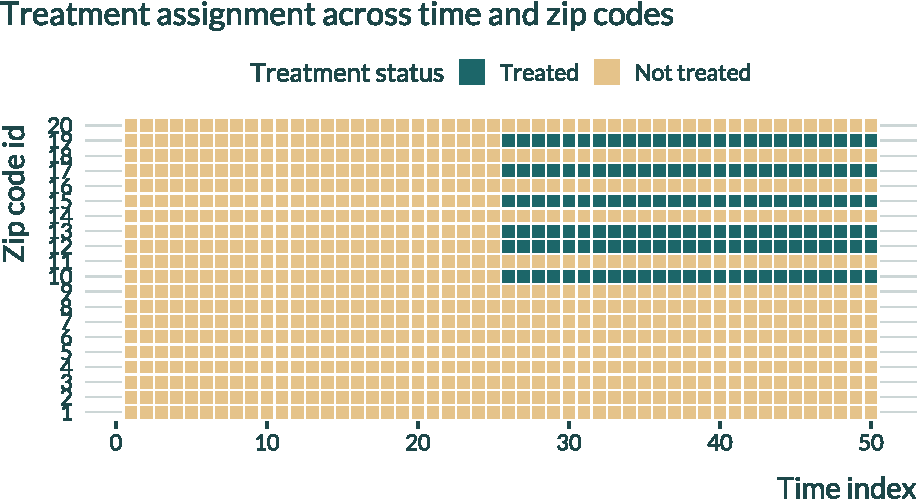
\includegraphics[width=0.85\linewidth]{images/treatment_allocation_DID-1} \end{center}

\hypertarget{quick-data-exploration}{%
\paragraph{Quick data exploration}\label{quick-data-exploration}}

I quickly explore a generated data set to get a sense of how the data is
distributed. First, I display the distribution of potential outcomes.

\begin{center}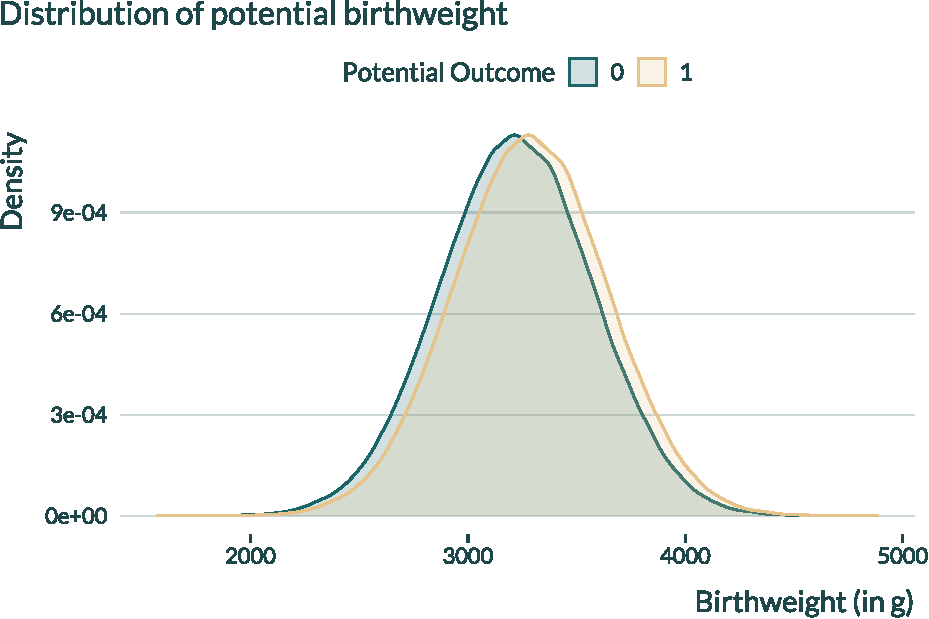
\includegraphics[width=0.85\linewidth]{images/eda_distrib_outcome-1} \end{center}

Then, I compare the average birthweight before and after the treatment,
in the control and treatment group.

\begin{center}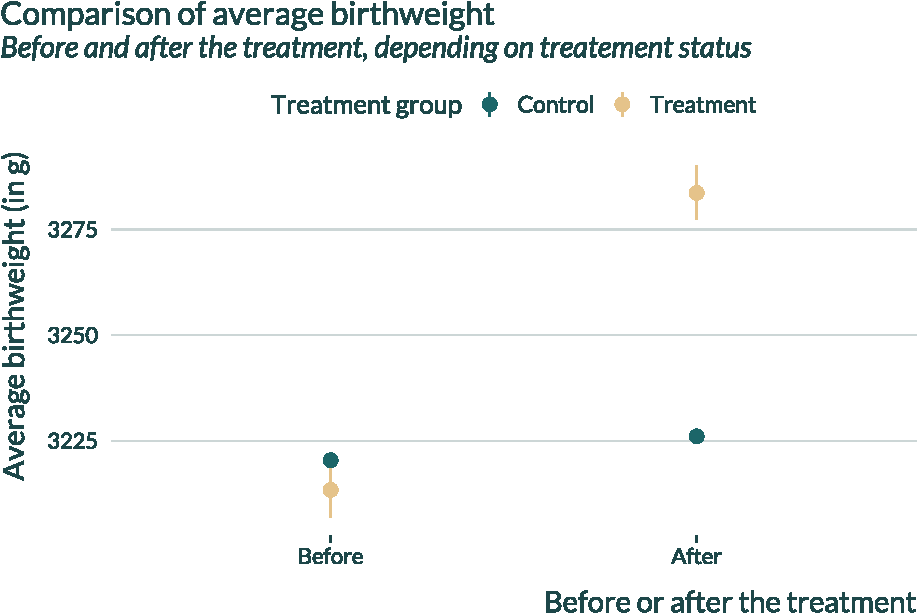
\includegraphics[width=0.85\linewidth]{images/eda_comparison_treatment-1} \end{center}

\hypertarget{estimation}{%
\subsubsection{Estimation}\label{estimation}}

I then define a function to run the estimation.

\begin{Shaded}
\begin{Highlighting}[]
\NormalTok{estimate\_DID }\OtherTok{\textless{}{-}} \ControlFlowTok{function}\NormalTok{(data) \{}
\NormalTok{  reg }\OtherTok{\textless{}{-}}\NormalTok{ data }\SpecialCharTok{\%\textgreater{}\%} 
    \FunctionTok{mutate}\NormalTok{(}
      \AttributeTok{zip =} \FunctionTok{as.factor}\NormalTok{(zip),}
      \AttributeTok{t =} \FunctionTok{as.factor}\NormalTok{(t),}
      \AttributeTok{treated =} \FunctionTok{as.numeric}\NormalTok{(treated),}
      \AttributeTok{in\_treatment =} \FunctionTok{as.numeric}\NormalTok{(in\_treatment),}
      \AttributeTok{t\_centered =} \FunctionTok{as.factor}\NormalTok{(t\_centered)}
\NormalTok{    ) }\SpecialCharTok{\%\textgreater{}\%} 
    \FunctionTok{feols}\NormalTok{(}
      \AttributeTok{data =}\NormalTok{ ., }
      \AttributeTok{fml =}\NormalTok{ birthweight }\SpecialCharTok{\textasciitilde{}}\NormalTok{ treated }\SpecialCharTok{|}\NormalTok{ zip }\SpecialCharTok{+}\NormalTok{ t}
\NormalTok{    ) }\SpecialCharTok{\%\textgreater{}\%} 
\NormalTok{    broom}\SpecialCharTok{::}\FunctionTok{tidy}\NormalTok{() }\SpecialCharTok{\%\textgreater{}\%} 
    \FunctionTok{rename}\NormalTok{(}\AttributeTok{p\_value =}\NormalTok{ p.value, }\AttributeTok{se =}\NormalTok{ std.error) }\SpecialCharTok{\%\textgreater{}\%} 
    \FunctionTok{select}\NormalTok{(}\SpecialCharTok{{-}}\NormalTok{statistic) }
    \CommentTok{\# suppressMessages() \#Warning saying that NA values dropped and }
    \CommentTok{\# \#that one or two factors are removed due to colinearity}
  
  \FunctionTok{return}\NormalTok{(reg)}
\NormalTok{\}}
\end{Highlighting}
\end{Shaded}

Here is an example of an output of this function:

\begin{longtable}[]{@{}lrrr@{}}
\toprule\noalign{}
term & estimate & se & p\_value \\
\midrule\noalign{}
\endhead
\bottomrule\noalign{}
\endlastfoot
treated & 81.9236 & 9.613534 & 0 \\
\end{longtable}

\hypertarget{one-simulation}{%
\subsubsection{One simulation}\label{one-simulation}}

Note that to run power calculations, we need to have access to the true
effects which are not directly input parameters. Therefore, before
running the estimation, I write a short function to compute the average
treatment effect on the treated (ATET). I will add this information to
the estimation results.

\begin{Shaded}
\begin{Highlighting}[]
\NormalTok{compute\_true\_effect\_DID }\OtherTok{\textless{}{-}} \ControlFlowTok{function}\NormalTok{(data) \{}
\NormalTok{  data }\SpecialCharTok{\%\textgreater{}\%} 
    \FunctionTok{filter}\NormalTok{(treated) }\SpecialCharTok{\%\textgreater{}\%} 
    \FunctionTok{summarise}\NormalTok{(}\AttributeTok{true\_effect =} \FunctionTok{mean}\NormalTok{(birthweight1 }\SpecialCharTok{{-}}\NormalTok{ birthweight0)) }\SpecialCharTok{\%\textgreater{}\%} 
\NormalTok{    .}\SpecialCharTok{$}\NormalTok{true\_effect}
\NormalTok{\}  }
\end{Highlighting}
\end{Shaded}

We can now run a simulation, combining \texttt{generate\_data\_DID} and
\texttt{estimate\_DID}. To do so I create the function
\texttt{compute\_sim\_DID}. This simple function takes as input the
various parameters. It returns a table with the estimate of the
treatment, its p-value and standard error, the true effect and the
proportion of treated units. Note that for now, I do not store the
values of the other parameters for simplicity because I consider them
fixed over the study.

Here is an example of an output of this function.

\begin{longtable}[]{@{}lrrrrrrr@{}}
\toprule\noalign{}
term & estimate & se & p\_value & N\_z & N\_t & p\_treat &
true\_effect \\
\midrule\noalign{}
\endhead
\bottomrule\noalign{}
\endlastfoot
treated & 68.90676 & 9.615794 & 0 & 5000 & 24 & 0.05 & 65 \\
\end{longtable}

\hypertarget{all-simulations}{%
\subsubsection{All simulations}\label{all-simulations}}

I will run the simulations for different sets of parameters by looping
the \texttt{compute\_sim\_DID} function over the set of parameters. I
thus create a table with all the values of the parameters to test,
\texttt{param\_DID}. Note that in this table each set of parameters
appears \texttt{N\_iter} times as we want to run the analysis
\(n_{iter}\) times for each set of parameters.

\begin{Shaded}
\begin{Highlighting}[]
\NormalTok{vect\_p\_treat }\OtherTok{\textless{}{-}} \FunctionTok{c}\NormalTok{(}\FloatTok{0.001}\NormalTok{, }\FunctionTok{seq}\NormalTok{(}\FloatTok{0.002}\NormalTok{, }\FloatTok{0.01}\NormalTok{, }\FloatTok{0.002}\NormalTok{), }\FunctionTok{c}\NormalTok{(}\FloatTok{0.01}\NormalTok{, }\FloatTok{0.02}\NormalTok{, }\FloatTok{0.03}\NormalTok{))}
\NormalTok{N\_iter }\OtherTok{\textless{}{-}} \DecValTok{100}

\NormalTok{param\_DID }\OtherTok{\textless{}{-}}\NormalTok{ baseline\_param\_DID }\SpecialCharTok{\%\textgreater{}\%} 
  \FunctionTok{select}\NormalTok{(}\SpecialCharTok{{-}}\NormalTok{p\_treat) }\SpecialCharTok{\%\textgreater{}\%} 
  \FunctionTok{crossing}\NormalTok{(vect\_p\_treat) }\SpecialCharTok{\%\textgreater{}\%} 
  \FunctionTok{rename}\NormalTok{(}\AttributeTok{p\_treat =}\NormalTok{ vect\_p\_treat) }\SpecialCharTok{\%\textgreater{}\%} 
  \FunctionTok{crossing}\NormalTok{(}\AttributeTok{rep\_id =} \DecValTok{1}\SpecialCharTok{:}\NormalTok{N\_iter) }\SpecialCharTok{\%\textgreater{}\%} 
  \FunctionTok{select}\NormalTok{(}\SpecialCharTok{{-}}\NormalTok{rep\_id)}
\end{Highlighting}
\end{Shaded}

I then run the simulations by looping our \texttt{compute\_sim\_IV}
function on \texttt{param\_IV} using the \texttt{purrr} package
(\texttt{pmap\_dfr} function).

\begin{Shaded}
\begin{Highlighting}[]
\FunctionTok{tic}\NormalTok{()}
\NormalTok{sim\_DID }\OtherTok{\textless{}{-}} \FunctionTok{pmap\_dfr}\NormalTok{(param\_DID, compute\_sim\_DID)}
\FunctionTok{beep}\NormalTok{()}
\FunctionTok{toc}\NormalTok{()}

\CommentTok{\# saveRDS(sim\_DID, here("Outputs/sim\_DID.RDS"))}
\end{Highlighting}
\end{Shaded}

\hypertarget{analysis-of-the-results}{%
\subsection{Analysis of the results}\label{analysis-of-the-results}}

\hypertarget{quick-exploration}{%
\subsubsection{Quick exploration}\label{quick-exploration}}

First, I quickly explore the results. I plot the distribution of the
estimated effect sizes, along with the true effect. The estimator is
unbiased and recover, on average, the true effect:

\begin{center}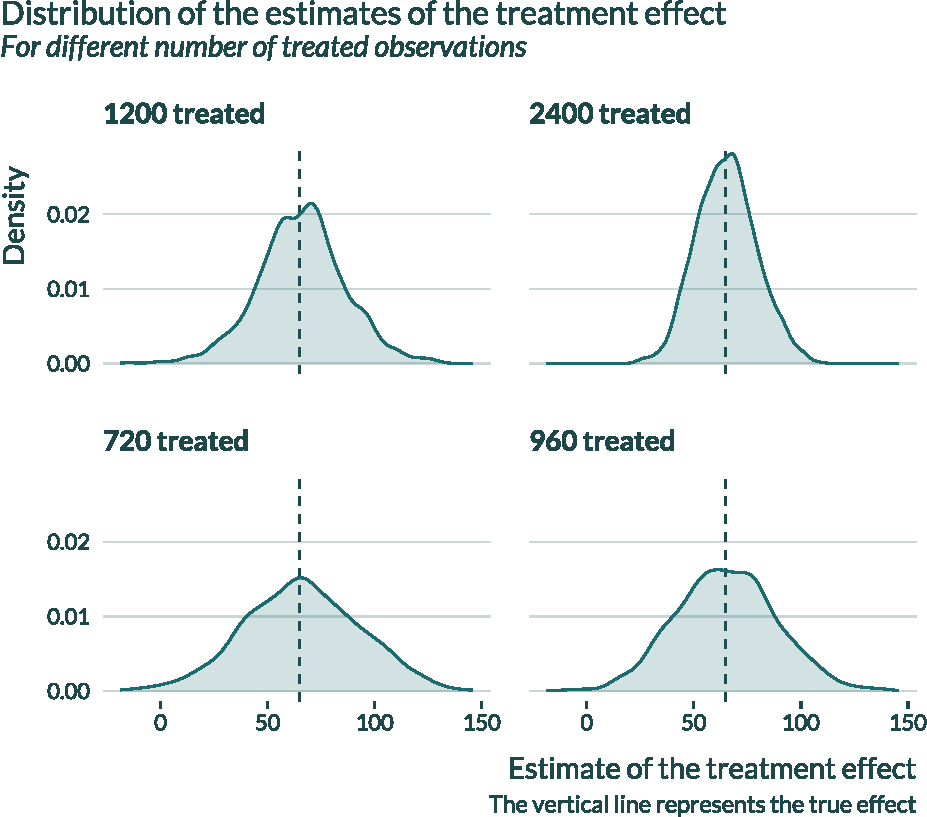
\includegraphics[width=0.85\linewidth]{images/exploration_results_DID-1} \end{center}

\hypertarget{computing-bias-and-exaaggeration-ratio}{%
\subsubsection{Computing bias and exaaggeration
ratio}\label{computing-bias-and-exaaggeration-ratio}}

We want to compare \(\mathbb{E}[\beta_0/\widehat{\beta}]\) and
\(\mathbb{E}[\beta_0/ \widehat{\beta}|signif]\). The first term
represents the bias and the second term represents the exaggeration
ratio. These terms depend on the true effect size.

\begin{Shaded}
\begin{Highlighting}[]
\NormalTok{summarise\_sim\_DID }\OtherTok{\textless{}{-}} \ControlFlowTok{function}\NormalTok{(data) \{}
\NormalTok{  data }\SpecialCharTok{\%\textgreater{}\%}
    \FunctionTok{mutate}\NormalTok{(}\AttributeTok{significant =}\NormalTok{ (p\_value }\SpecialCharTok{\textless{}=} \FloatTok{0.05}\NormalTok{)) }\SpecialCharTok{\%\textgreater{}\%} 
    \FunctionTok{group\_by}\NormalTok{(p\_treat, N\_z, N\_t) }\SpecialCharTok{\%\textgreater{}\%}
    \FunctionTok{summarise}\NormalTok{(}
      \AttributeTok{power =} \FunctionTok{mean}\NormalTok{(significant, }\AttributeTok{na.rm =} \ConstantTok{TRUE}\NormalTok{)}\SpecialCharTok{*}\DecValTok{100}\NormalTok{, }
      \AttributeTok{type\_m =} \FunctionTok{mean}\NormalTok{(}\FunctionTok{ifelse}\NormalTok{(significant, }\FunctionTok{abs}\NormalTok{(estimate}\SpecialCharTok{/}\NormalTok{true\_effect), }\ConstantTok{NA}\NormalTok{), }\AttributeTok{na.rm =} \ConstantTok{TRUE}\NormalTok{),}
      \AttributeTok{exag\_ratio =} \FunctionTok{mean}\NormalTok{(}\FunctionTok{ifelse}\NormalTok{(significant, estimate}\SpecialCharTok{/}\NormalTok{true\_effect, }\ConstantTok{NA}\NormalTok{), }\AttributeTok{na.rm =} \ConstantTok{TRUE}\NormalTok{),}
      \AttributeTok{bias\_all =} \FunctionTok{mean}\NormalTok{(estimate}\SpecialCharTok{/}\NormalTok{true\_effect, }\AttributeTok{na.rm =} \ConstantTok{TRUE}\NormalTok{),}
      \AttributeTok{bias\_all\_median =} \FunctionTok{median}\NormalTok{(estimate}\SpecialCharTok{/}\NormalTok{true\_effect, }\AttributeTok{na.rm =} \ConstantTok{TRUE}\NormalTok{),}
      \AttributeTok{.groups   =} \StringTok{"drop"}
\NormalTok{    ) }\SpecialCharTok{\%\textgreater{}\%} 
    \FunctionTok{ungroup}\NormalTok{() }\SpecialCharTok{\%\textgreater{}\%} 
    \FunctionTok{mutate}\NormalTok{(}\AttributeTok{n\_treated =}\NormalTok{ p\_treat}\SpecialCharTok{*}\NormalTok{N\_z}\SpecialCharTok{*}\NormalTok{N\_t)}
\NormalTok{\} }

\NormalTok{summary\_sim\_DID }\OtherTok{\textless{}{-}} \FunctionTok{summarise\_sim\_DID}\NormalTok{(sim\_DID)}
\CommentTok{\# saveRDS(summary\_sim\_DID, here("Outputs/summary\_sim\_DID.RDS"))}
\end{Highlighting}
\end{Shaded}

\hypertarget{main-graph}{%
\subsubsection{Main graph}\label{main-graph}}

To analyze our results, we build a unique and simple graph:

\begin{center}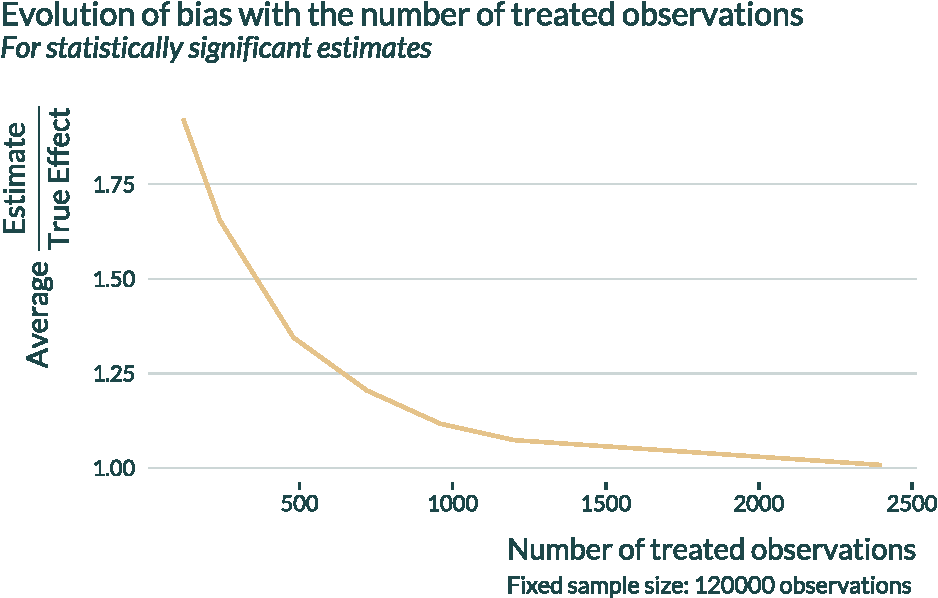
\includegraphics[width=0.85\linewidth]{images/main_graph_DID-1} \end{center}

<!--radix_placeholder_site_after_body-->
<!--/radix_placeholder_site_after_body-->

<!--radix_placeholder_navigation_after_body-->
<!--/radix_placeholder_navigation_after_body-->

\end{document}
